This appendix is a post-reflection on how the uncertainty impacts our results.

All our measures were made in rounded seconds, this means that all our data suffer from an uncertainty that could impact the results and the conclusions made. We will compute the uncertainty and re-plot the speedups that were used in this report, but this time showing the uncertainty.

First, let's find the formula giving the uncertainty. For a single measured value, say 10 seconds, we know that is has been rounded. It could be in reality 10.1 seconds, 10.5 seconds or, the maximum, 10.999999 seconds. Thus, the measure could be in reality from 10 seconds to 10.9999 seconds. Therefor, we have an uncertainty of maximum +1 seconds.

Based on this principle, we computed the uncertainty of the speedup ($S$) based on two measures ($x_1$, $x_2$) :

\[ S = \frac{x_1}{x_2} \]

\[ S_{max} = \frac{x_1+1}{x_2} \]

\[ S_{min} = \frac{x_1}{x_2+1} \]

\[ S_{uncertainty} = S_{max} - S_{min} = \frac{x_1+1}{x_2} - \frac{x_1}{x_2+1} = \frac{x_1+x_2+1}{x_2^2+x_2} \]

Given the previous formula, we re-plotted the speedup with the uncertainty. Figures \ref{fig: plot both matrix uncertain} and \ref{fig: plot both leven uncertain} show speedups of Aparapi and JCuda on the matrix multiplication and Levenshtein distance respectively with the uncertainty. We can see that the uncertainty should explain why the plots are not regular and smooth. Fortunately for us, the uncertainty is not great enough to impact the conclusions made. JCuda is still faster on most cases than Aparapi, even taking into account the incertainty.

\begin{figure}[H]
\centering
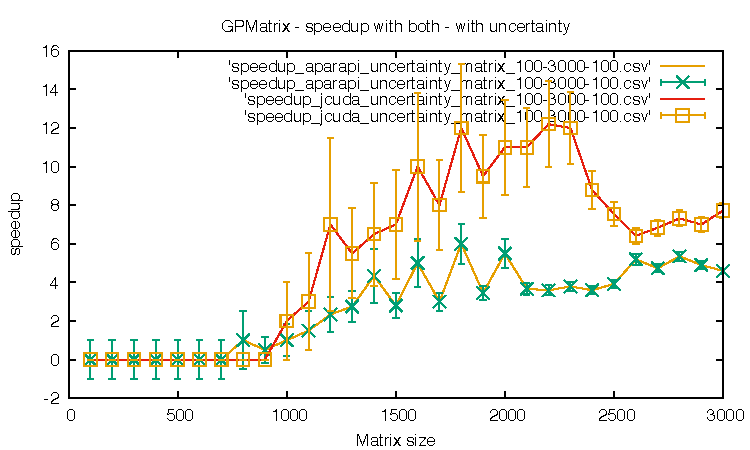
\includegraphics[width=1\textwidth]{speedup_both_uncertainty_matrix-5x.pdf}
\caption{Speedup of both Aparapi and JCuda on the matrix multiplication, showing uncertainty}
\label{fig: plot both matrix uncertain}
\end{figure}

\begin{figure}[H]
\centering
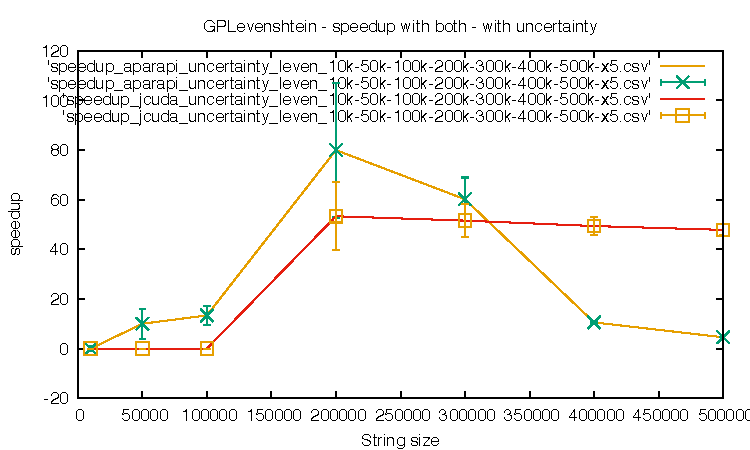
\includegraphics[width=1\textwidth]{speedup_both_uncertainty_leven-5x.pdf}
\caption{Speedup of both Aparapi and JCuda on the Levenstein distance computation, showing uncertainty}
\label{fig: plot both leven uncertain}
\end{figure}